\documentclass{article}
\usepackage{graphicx}
\usepackage[utf8]{inputenc}
\usepackage{amsmath, amssymb, latexsym}
\usepackage{neuralnetwork}
\usepackage{multicol}

\usepackage{pgfplots}
\usepackage{algorithm}
\usepackage[noend]{algpseudocode}
\usepackage{tikz}
\usepackage{nicefrac}
\pgfplotsset{every axis legend/.append style={
at={(0,0)},
anchor=north east}}
\usetikzlibrary{shapes,positioning,intersections,quotes}
\usetikzlibrary{arrows.meta,
                bending,
                intersections,
                quotes,
                shapes.geometric}
                
\definecolor{darkgreen}{rgb}{0.0, 0.6, 0.0}
\definecolor{darkred}{rgb}{0.7, 0.0, 0.0}
\makeatletter
\def\BState{\State\hskip-\ALG@thistlm}
\makeatother
\title{Week 8}
\begin{document}
\pagenumbering{gobble}
\maketitle
\newpage
\pagenumbering{arabic}

\section*{Why do we need neural networks?}
\begin{itemize}
  \item We can have complex data sets with many (1000's) important features.
  \item Using logistic regression becomes expensive really fast.
  \item The only way to get around this is to use a subset of features. This, however, may result in less accuracy.
\end{itemize}

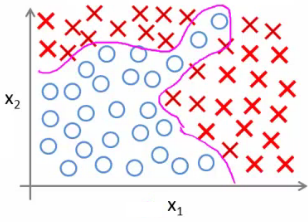
\includegraphics[width=0.5\textwidth]{resources/many_features_classifier}

\subsection*{Problems where n is large - computer vision}
\begin{itemize}
  \item Computer vision sees a matrix of pixel intensity values.
  \item To build a car detector: Build a training set of cars and not cars. Then test against a car.
  \item Plot two pixels (two pixel locations) and car or not car on the graph.
\end{itemize}

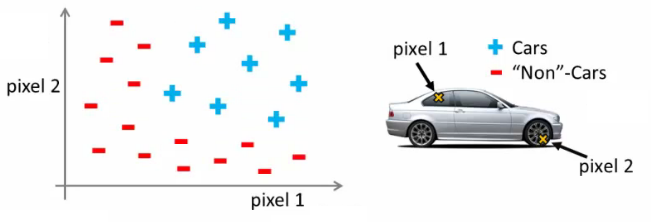
\includegraphics[width=0.8\textwidth]{resources/cars}

~\\Feature space
\subsection*{Problems where n is large - computer vision}
\begin{itemize}
  \item If we used 50 x 50 pixels $-->$ 2500 pixels, so n = 2500.
  \item If RGB then 7500.
  \item If 100 x 100 RB then $-->$ 50 000 000 features.
  \item Way too big.
\end{itemize}

\section*{Neurons and the brain}

\begin{itemize}
  \item The desire to construct computers that mimicked brain activities drove the creation of neural networks (NNs).
  \item Used a lot in the 80s. Popularity diminished in 90s.
  \item Large-scale neural networks have just recently become computationally feasible due to the computational cost of NNs.
\end{itemize}

\subsection*{Brain}

\begin{itemize}
  \item Hypothesis is that the brain has a single learning algorithm.
  \item If the optic nerve is rerouted to the auditory cortex, the auditory cortex is learns to see.
  \item If you rewrite the optic nerve to the somatosensory cortex then it learns to see.
\end{itemize}

\section*{Model representation I}

Neuron:
\begin{itemize}
  \item Cell body
  \item Number of input wires (dendrites)
  \item Output wire (axon)
\end{itemize}

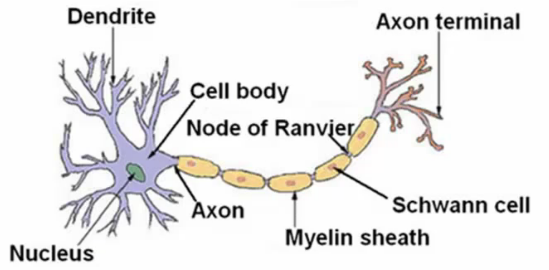
\includegraphics[width=0.8\textwidth]{resources/neuron}

\begin{itemize}
  \item Neurone gets one or more inputs through dendrites.
  \item Does processing.
  \item The output is sent along the axon.
  \item Neurons communicate through electric spikes.
\end{itemize}

\subsection*{Artificial neural network - representation of a neurone}

\begin{itemize}
  \item Feed input via input wires.
  \item Logistic unit does computation.
  \item Sends output down output wires.
\end{itemize}

\begin{multicols}{2}

  \begin{neuralnetwork}[height=4]
    \newcommand{\x}[2]{$x_#2$}
    \newcommand{\y}[2]{$h_{\theta}(x)$}
    \inputlayer[count=3, bias=true, title=Input\\layer, text=\x]
    \outputlayer[count=1, title=Output\\layer, text=\y] \linklayers
  \end{neuralnetwork}

  \columnbreak

  \begin{align*}
    x & = \begin{bmatrix}
      x_{0} \\
      x_{1} \\
      x_2   \\
      x_3
    \end{bmatrix}
  \end{align*}


  \begin{align*}
    \theta & = \begin{bmatrix}
      \theta_{0} \\
      \theta_{1} \\
      \theta_2   \\
      \theta_3
    \end{bmatrix}
  \end{align*}
\end{multicols}

\begin{itemize}
  \item The diagram above represents a single neurone.
  \item $x_0$ is called the bias unit.
  \item $\theta$ vector is called the weights of a model.
\end{itemize}

\begin{neuralnetwork}[height=4]
  \newcommand{\x}[2]{$x_#2$}
  \newcommand{\h}[2]{\small $a^{(1)}_#2$}
  \newcommand{\y}[2]{$h_{\theta}(x)$}
  \inputlayer[count=3, bias=true, title=Input\\layer, text=\x]
  \hiddenlayer[count=3, bias=true, title=Hidden\\layer, text=\h] \linklayers
  \outputlayer[count=1, title=Output\\layer, text=\y] \linklayers
\end{neuralnetwork}

\begin{itemize}
  \item First layer is the input layer.
  \item Final layer is the output layer - produces value computed by a hypothesis.
  \item Middle layer(s) are called the hidden layers.
  \item You don't observe the values processed in the hidden layer.
  \item Every input/activation goes to every node in following layer.
\end{itemize}

$$a^{(2)}_1 = g(\Theta^{(1)}_{10}x_0+\Theta^{(1)}_{11}x_1+\Theta^{(1)}_{12}x_2+\Theta^{(1)}_{13}x_3)$$
$$a^{(2)}_2 = g(\Theta^{(1)}_{20}x_0+\Theta^{(1)}_{21}x_1+\Theta^{(1)}_{22}x_2+\Theta^{(1)}_{23}x_3)$$
$$a^{(2)}_1 = g(\Theta^{(1)}_{30}x_0+\Theta^{(1)}_{31}x_1+\Theta^{(1)}_{32}x_2+\Theta^{(1)}_{33}x_3)$$
$$h_{\Theta}(x) = g(\Theta^{(2)}_{10}a^{(2)}_0+\Theta^{(2)}_{11}a^{(2)}_1+\Theta^{(2)}_{12}a^{(2)}_2+\Theta^{(2)}_{13}a^{(2)}_3)$$

\section*{Model representation II}
In this section, we'll look at how to do the computation efficiently using a vectorized approach. We'll also look at why NNs are useful and how we can use them to learn complicated nonlinear things.

~\\
Let's define a few more terms:

$$z^{(2)}_1 = \Theta^{(1)}_{10}x_0+\Theta^{(1)}_{11}x_1+\Theta^{(1)}_{12}x_2+\Theta^{(1)}_{13}x_3$$

~\\
We can now write:
$$a^{(2)}_1 = g(z^{(2)}_1)$$

\begin{multicols}{4}

  \begin{align*}
    x & = \begin{bmatrix}
      x_{0} \\
      x_{1} \\
      x_2   \\
      x_3
    \end{bmatrix}
  \end{align*}

  \columnbreak

  \begin{align*}
    z^{(2)} & = \begin{bmatrix}
      z^{(2)}_1 \\
      z^{(2)}_2 \\
      z^{(2)}_3
    \end{bmatrix}
  \end{align*}
  \columnbreak
  \columnbreak
\end{multicols}


\begin{itemize}
  \item $z^{(2)}$ is a $3x1$ vector.
  \item $a^{(2)}$ ia also a $3x1$ vector.
  \item Middle layer(s) are called the hidden layers.
  \item $g()$ applies the sigmoid (logistic) function element wise to each member of the $z^{(2)}$ vector.
  \item Obviously the "activation" for the input layer is just the input!
  \item $a^{(1)}$ is the vector of inputs.
  \item $a^{(2)}$ is the vector of values calculated by the $g(z^{(2)})$ function.
  \item We send our input values to the hidden layers and let them learn which values produce the best final result to feed into the final output layer.
  \item This process is also called forward propagation.
\end{itemize}

~\\
Other architectural designs are also possible:\\
\begin{itemize}
  \item More/less nodes per layer.
  \item More layers.
\end{itemize}

\begin{neuralnetwork}[height=4]
  \newcommand{\x}[2]{$x_#2$}
  \newcommand{\hfirst}[2]{\small $a^{(1)}_#2$}
  \newcommand{\hsecond}[2]{\small $a^{(2)}_#2$}
  \newcommand{\y}[2]{$h_{\theta}(x)$}
  \inputlayer[count=3, bias=true, title=Input\\layer, text=\x]
  \hiddenlayer[count=3, bias=true, title=Hidden\\layer, text=\hfirst] \linklayers\\
  \hiddenlayer[count=2, bias=true, title=Hidden\\layer, text=\hsecond] \linklayers
  \outputlayer[count=1, title=Output\\layer, text=\y] \linklayers
\end{neuralnetwork}

~\\
Layer 2 has three hidden units (plus bias), layer 3 has two hidden units (plus bias), and by the time you get to the output layer, you have a really intriguing non-linear hypothesis.

\section*{AND function}

\begin{neuralnetwork}[height=3]
  \newcommand{\x}[2]{$x_#2$}
  \newcommand{\y}[2]{$h_{\theta}(x)$}
  \inputlayer[count=2, bias=true, title=Input\\layer, text=\x]
  \outputlayer[count=1, title=Output\\layer, text=\y] \linklayers
\end{neuralnetwork}

~\\
Let $x_0 = 1$ and theta vector be:

\begin{align*}
  \Theta^{(1)}_1 & = \begin{bmatrix}
    -30 \\
    20  \\
    20
  \end{bmatrix}
\end{align*}

Then hypothesis is:

$$h_{\Theta}(x) = g(-30 \cdot 1 + 20 \cdot x_1 + 20 \cdot x_2)$$

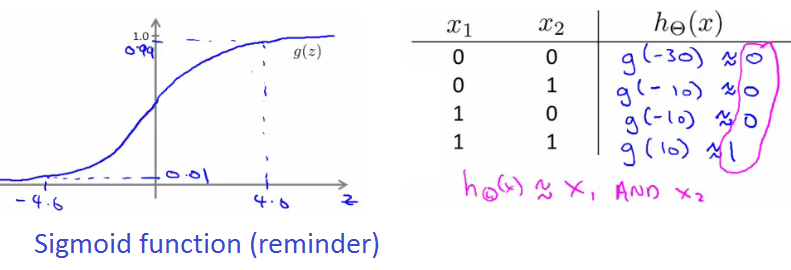
\includegraphics[width=\textwidth]{resources/sigmoid}

\section*{XNOR function}
~\\
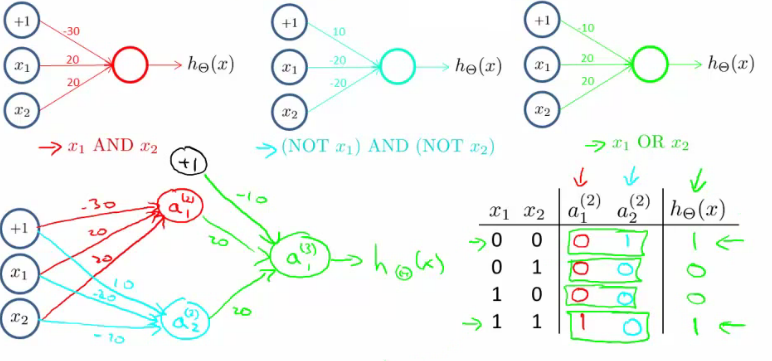
\includegraphics[width=\textwidth]{resources/xnor}

\end{document}